\documentclass{sysuthesis}

%%
% 论文相关信息
% 本文档中前缀"c-"代表中文版字段, 前缀"e-"代表英文版字段
% modifyer: 黄俊杰(huangjj27, 349373001dc@gmail.com)
% update date: 2017-04-13
%%

% 标题
% 论文题目应以简短、明确的词语恰当概括整个论文的核心内容,避免使用不常见的缩略词、缩写字。读者通过标题可大致了解毕业设计(论文)的内容、专业的特点和科学的范畴。中文题目一般不宜超过 24 个字,必要时可增加副标题。外文题目一般不宜超过 12 个实词

% 封面标题。由于技术所限,封面题目过长的划分交由用户您进行定夺
% 这也能让您的论文封面看起来更有美感
\covertitlefirst{中山大学}
\covertitlesecond{本科毕业论文(设计)}

% Author:   Souler Ou
% 修改者:    欧一锋
% Date:     3/30/2018
% Mail:     ou@souler.cc
%如果英文标题过长可以使用此两项作为表三(答辩记录表)的标题。
\etitlefirst{\LaTeX \ Template}
\etitlesecond{for SYSU Graduation Thesis}

% 中文标题
\ctitle{中山大学本科毕业论文}
\etitle{ \LaTeX \ Template for SYSU Graduation Thesis}

% 作者详细信息
\author{王小明}
\cauthor{王\ 小\ 明}    % 封面作者
\eauthor{Wang Xiaoming}
\studentid{12350004}
\cschool{计算机学院}

\cmajor{计算机科学与技术}
\emajor{Computer Science and Technology}

% 指导老师
\cmentor{王大明 \ (教授)}
\ementor{Prof. 王大明}

   % 论文相关信息
%%
% 摘要信息
% 本文档中前缀"c-"代表中文版字段, 前缀"e-"代表英文版字段
% 摘要内容应概括地反映出本论文的主要内容,主要说明本论文的研究目的、内容、方法、成果和结论。要突出本论文的创造性成果或新见解,不要与引言相 混淆。语言力求精练、准确,以 300—500 字为宜。
% 在摘要的下方另起一行,注明本文的关键词(3—5 个)。关键词是供检索用的主题词条,应采用能覆盖论文主要内容的通用技术词条(参照相应的技术术语 标准)。按词条的外延层次排列(外延大的排在前面)。摘要与关键词应在同一页。
% modifier: 黄俊杰(huangjj27, 349373001dc@gmail.com)
% update date: 2017-04-15
%%

\cabstract{
摘要内容应概括地反映出本论文的主要内容,主要说明本论文的研究目的、内容、方法、成果和结论。要突出本论文的创造性成果或新见解,不要与引言相混淆。语言力求精练、准确,以300—500字为宜。在摘要的下方另起一行,注明本文的关键词(3—5个)。关键词是供检索用的主题词条,应采用能覆盖论文主要内容的通用技术词条(参照相应的技术术语标准)。按词条的外延层次排列(外延大的排在前面)。摘要与关键词应在同一页。
}
% 中文关键词(每个关键词之间用“;”分开,最后一个关键词不打标点符号。)
\ckeywords{本科毕业论文;\LaTeX\ 模板;中山大学}

\eabstract{
英文摘要内容与中文摘要相同,以250—400个实词为宜。摘要下方另起一行注明英文关键词(Keywords3—5个)。
}
% 英文文关键词(每个关键词之间用半角加空格分开, 最后一个关键词不打标点符号。)
\ekeywords{undergraduate thesis, \LaTeX\ template, Sun Yat-Sen University}

   % 摘要内容

\begin{document}
  % 论文前置部分
  \frontmatter
    \pagenumbering{Roman}
    \maketitle  % 封面
    \clearemptydoublepage   % 空白页
    % 开题报告
    % 过程检查记录表
    % 答辩情况等级表
    \makedisclaim   % 学术诚信声明
    \makeabstract   % 中英文摘要
    \tableofcontents    % 目录
    \makelistoffiguretable

  % 论文主体部分
  \mainmatter
    % 引言

    % 正文
    %%
% 引言或背景
% 引言是论文正文的开端,应包括毕业论文选题的背景、目的和意义;对国内外研究现状和相关领域中已有的研究成果的简要评述;介绍本项研究工作研究设想、研究方法或实验设计、理论依据或实验基础;涉及范围和预期结果等。要求言简意赅,注意不要与摘要雷同或成为摘要的注解。
% modifier: 黄俊杰(huangjj27, 349373001dc@gmail.com)
% update date: 2017-04-15
%%

\chapter{绪论}
%定义,过去的研究和现在的研究,意义,与图像分割的不同,going deeper
\label{cha:introduction}
\section{选题背景与意义}
\label{sec:background}
% What is the problem
% why is it interesting and important
% Why is it hards, why do naive approaches fails
% why hasn't it been solved before
% what are the key components of my approach and results, also include any specific limitations,do not repeat the abstract
%contribution
引言是论文正文的开端,应包括毕业论文选题的背景、目的和意义;对国内外研究现状和相关领域中已有的研究成果的简要评述;介绍本项研究工作研究设想、研究方法或实验设计、理论依据或实验基础;涉及范围和预期结果等。要求言简意赅,注意不要与摘要雷同或成为摘要的注解。

\section{国内外研究现状和相关工作}
\label{sec:related_work}
对国内外研究现状和相关领域中已有的研究成果的简要评述。
\section{本文的论文结构与章节安排}

\label{sec:arrangement}

本文共分为六章,各章节内容安排如下:

第一章绪论。简单说明了本文章的选题背景与意义。

第二章为本科生毕业论文写作与印制规范。本章节就学校的规范,逐点进行描述,并给出来了相关例子说明本模板在格式上的正确性。

第三章为本模板的使用说明。

第四章为可用的\LaTeX 的代码段方便大家进行编辑。

第五、六章是本文的最后两章,作为空白章节例子。


    \chapter{毕业论文的撰写内容与要求}

\label{cha:sysu-thesis-contents-requirement}




    \chapter{\LaTeX 模板配置与使用}


\label{cha:sysu-thesis-latex-install-guide}

本部分内容将让你能够通过本\LaTeX 模板生成一份可用的pdf,并为后面修改源码撰写毕设做准备。

首先,我们会展示最简单的方法:直接使用overleaf进行编写。然后,我们整理了不同环境下\LaTeX 环境的配置指南与不同写作工具的配置技巧,方便各位同学使用本\LaTeX 模板。最后,我们说明了如何开始编写自己的毕业论文(设计)。


\section{使用Overleaf编写毕设}

Overleaf\footnote{网址可见\url{https://www.overleaf.com/}}是一个在线的Latex文档协作平台。我们不需要配置任何环境,便能够在上面直接使用本模板进行写作。操作步骤如下:

第一步,下载本项目压缩包(从\url{https://github.com/SYSU-SCC/sysu-thesis/releases}处下载即可),注意需要下载zip格式的压缩包。
然后,我们在Overleaf上新建项目,并上传该压缩包,可参考\autoref{fig:overleaf-new-proj}。


\begin{figure}[h]
	\centering
	\includegraphics[width=0.2\textwidth]{image/chap03/overleaf-create-proj.jpg}
	\includegraphics[width=0.7\textwidth]{image/chap03/overleaf-upload-proj.jpg}
	\caption{在Overleaf上创建并上传压缩包。}
	\label{fig:overleaf-new-proj}
\end{figure}

第二步,在Overleaf的菜单中调整编译工具为\texttt{xelatex},可参考\autoref{fig:overleaf-config}。

\begin{figure}[h]
	\centering
	\includegraphics[width=0.6\textwidth]{image/chap03/overleaf-config.jpg}
	\caption{在Overleaf上调整编译工具}
	\label{fig:overleaf-config}
\end{figure}


第三步,点击编译,得到本pdf,可以开始修改pdf了!最终可见\autoref{fig:overleaf-example}。


\begin{figure}[h]
	\centering
	\includegraphics[width=0.9\textwidth]{image/chap03/overleaf-example.jpg}
	\caption{Overleaf使用例子}
	\label{fig:overleaf-example}
\end{figure}



\section{编译环境配置}

编译环境配置相对来说比较简单,下载Tex Live2020并如同一般的程序一样安装即可。

\subsection{编译环境配置:Window篇}

在\url{https://mirrors.tuna.tsinghua.edu.cn/CTAN/systems/texlive/Images/}上下载Tex Live2020并参考教程\footnote{可以参考\url{https://zhuanlan.zhihu.com/p/58811994}}安装即可。

\subsection{编译环境配置:Linux篇}

在\url{https://mirrors.tuna.tsinghua.edu.cn/CTAN/systems/texlive/Images/}上下载Tex Live2020并参考教程\footnote{可以参考\url{https://zhuanlan.zhihu.com/p/55894177}}安装即可。


\subsection{编译环境配置:MacOS篇}

在MacOS上配置Latex的环境,这里我们使用的是MacTex。

\begin{enumerate}
	\item \url{https://www.tug.org/mactex/}下载MacTex安装。
	\item 安装步骤:不详细展开,按照图形界面点击即可, 傻瓜式安装。
\end{enumerate}

TIPS:MacTex文件比较大,有2G多,介意的话可以选择MacTex\_Basic包,只有100M以内,但是如果安装MacTex\_Basic,后期可能会遇到各种缺包的问题。


安装完成之后,可以简单测试一下安装是否成功。如可以查看Texshop应用是否安装好,或者在命令行测试一下\texttt{xelatex}命令是否可用。

\section{写作环境配置}

不同的写作工具对应不同的写作环境。这里我们给出几个工具的配置例子以供参考。

\subsection{模板编译流程}

由于\LaTeX 的限制,本模板需要经过四次编译才能生成完整的论文:

\begin{enumerate}
	\item 先使用xelatex编译一次
	\item 再使用bibtex编译一次
	\item 然后使用xelatex编译两次
\end{enumerate}

本编译流程已经写在Makefile中,修改模板源码后只需要执行\texttt{make pdf}即可按照该流程进行编译并生成最终的pdf。



\subsection{写作环境配置:Visual Studio Code}

Visual Studio Code是微软公司推出的轻量代码编辑器,我们可以做一些简单的配置,便可以用该编辑器修改我们的\LaTeX 模板,并实现一键编译。

\begin{enumerate}
	\item 安装 Visual Studio Code。
	\item 安装 LaTeX Workshop 插件。
\end{enumerate}

本项目的\texttt{.vscode/setting.json}下已经包含了与前面所述编译流程相同的配置。正常配置下,每次修改模板源码后按下保存(Ctrl+S),就能够自动进行编译产生pdf。效果图如\autoref{fig:vscode-example}所示。


\begin{figure}[h]
	\centering
	\includegraphics[width=\linewidth]{image/chap03/vscode-example.png}
	\caption{vscode配置好后的样例}
	\label{fig:vscode-example}
\end{figure}


\section{如何开始写毕业论文(设计)}

首先将所有个人信息,包括学号、姓名、专业、论文题目等,在\texttt{./docs/info.tex}中逐项进行更新。

然后我们再编辑\texttt{./docs/abstract.tex}补充论文摘要。

到了论文主体部分,我们可以自行编辑\texttt{./docs/chap01.tex},\texttt{./docs/chap02.tex}等文件进行编辑。如果章数不够,可以自行修改\texttt{main.tex}增加新的章节。

当论文主体编写完成后,我们再编辑\texttt{./docs/ack.tex}作为论文致谢。


% 首先将个人信息写到\texttt{./docs/info.tex}中。
    \chapter{简单的使用例子}
\label{cha:usage-example}

本部分将会根据毕设论文的写作需要,放置相关的例子和代码段供大家参考,方便大家的论文写作,如果更多有用的Latex使用例子也会欢迎提出PR,贡献更多的例子。

\section{图像的插入}

\subsection{文中的图像}
\begin{figure}
    \centering
    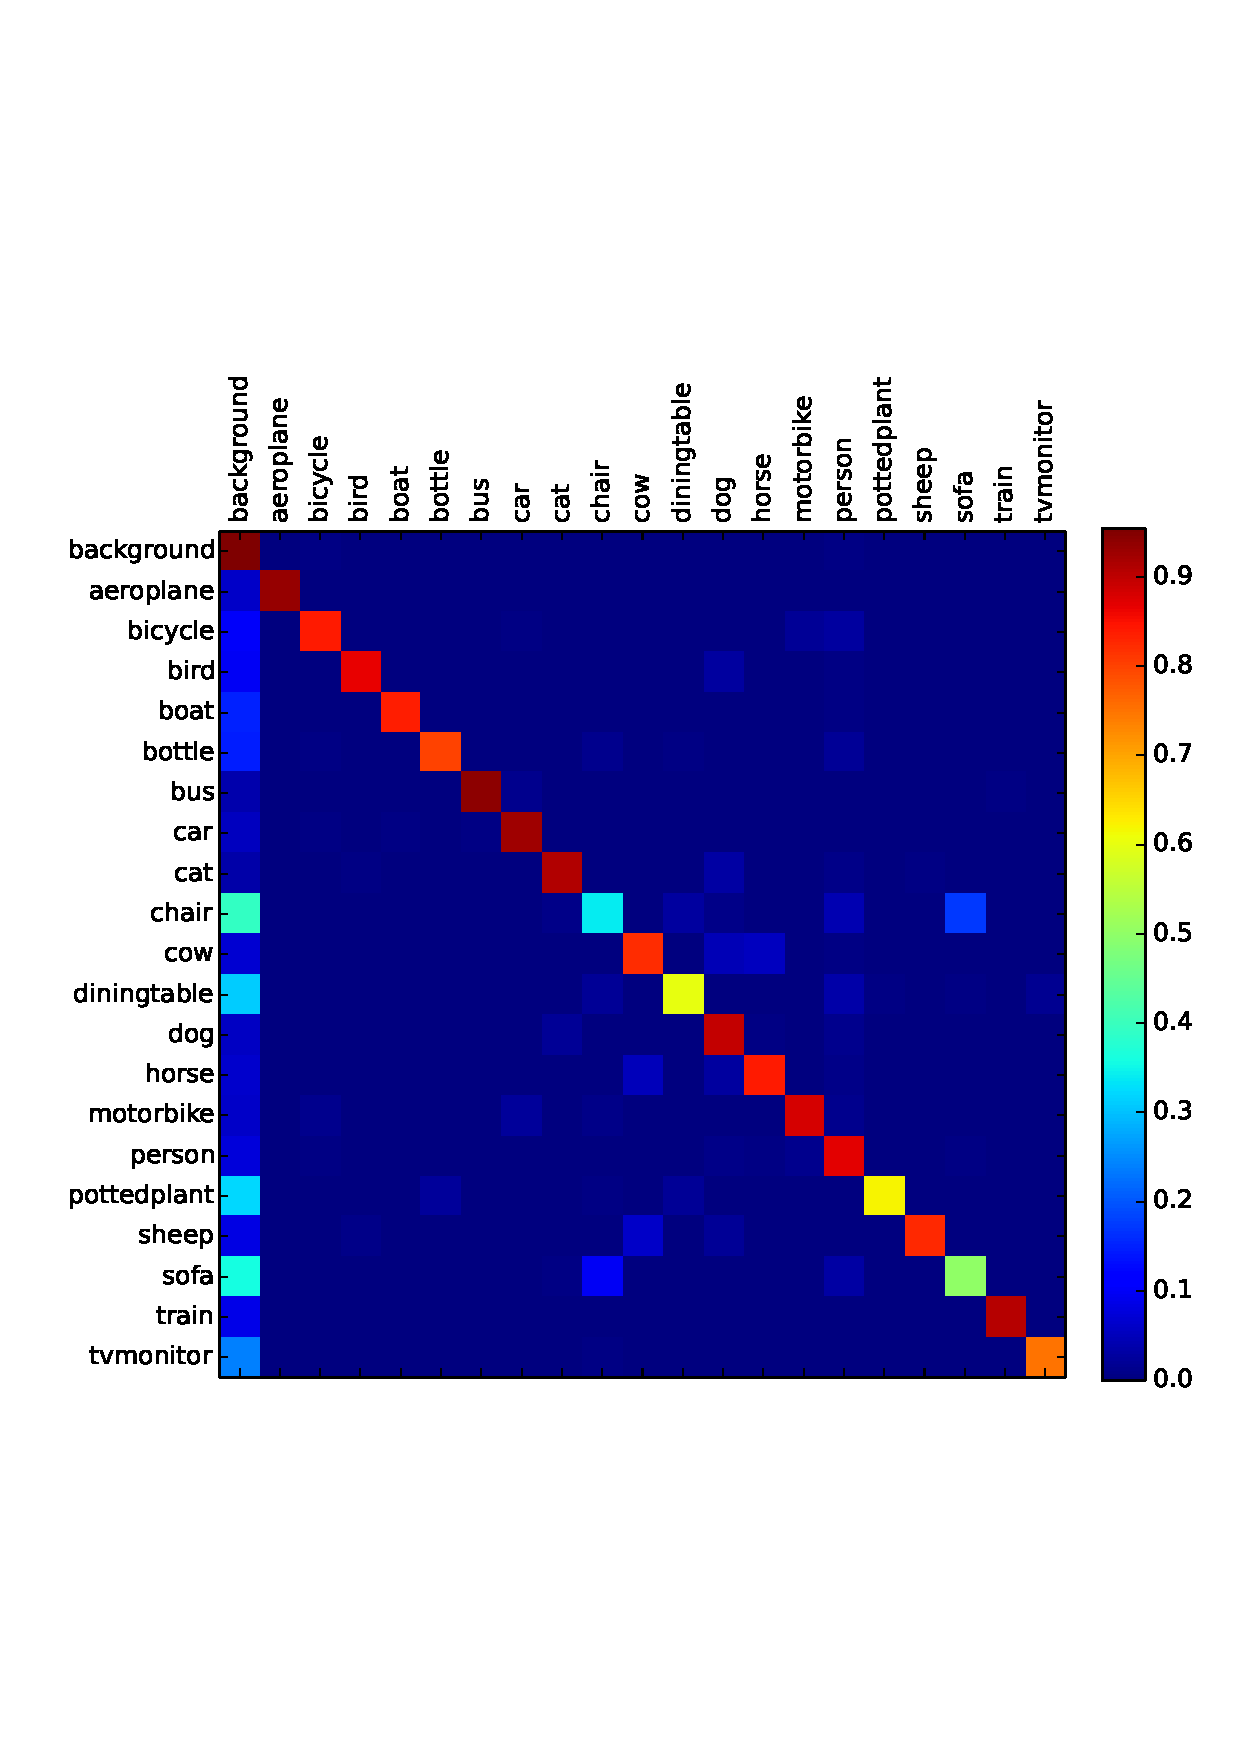
\includegraphics[width=0.5\textwidth]{image/chap04/confusion.pdf}
    \caption{文中的图像}
    \label{fig:image-embedding-text}
\end{figure}
论文主体是毕业论文的主要部分,必须言之成理,论据可靠,严格遵循本学科国际通行的学术规范。在写作上要注意结构合理、层次分明、重点突出,章节标题、公式图表符号必须规范统一。论文主体的内容根据不同学科有不同的特点,一般应包括以下几个方面: (1)毕业论文(设计)总体方案或选题的论证; (2)毕业论文(设计)各部分的设计实现,包括实验数据的获取、数据可行性及有效性的处理与分析、各部分的设计计算等; (3)对研究内容及成果的客观阐述,包括理论依据、创新见解、创造性成果及其改进与实际应用价值等; (4)论文主体的所有数据必须真实可靠,凡引用他人观点、方案、资料、数据等,无论曾否发表,无论是纸质或电子版,均应详加注释。自然科学论文应推理正确、结论清晰;人文和社会学科的论文应把握论点正确、论证充分、论据可靠,恰当运用系统分析和比较研究的方法进行模型或方案设计,注重实证研究和案例分析,根据分析结果提出建议和改进措施等。
论文主体是毕业论文的主要部分,必须言之成理,论据可靠,严格遵循本学科国际通行的学术规范。在写作上要注意结构合理、层次分明、重点突出,章节标题、公式图表符号必须规范统一。论文主体的内容根据不同学科有不同的特点,一般应包括以下几个方面: (1)毕业论文(设计)总体方案或选题的论证; (2)毕业论文(设计)各部分的设计实现,包括实验数据的获取、数据可行性及有效性的处理与分析、各部分的设计计算等; (3)对研究内容及成果的客观阐述,包括理论依据、创新见解、创造性成果及其改进与实际应用价值等; (4)论文主体的所有数据必须真实可靠,凡引用他人观点、方案、资料、数据等,无论曾否发表,无论是纸质或电子版,均应详加注释。自然科学论文应推理正确、结论清晰;人文和社会学科的论文应把握论点正确、论证充分、论据可靠,恰当运用系统分析和比较研究的方法进行模型或方案设计,注重实证研究和案例分析,根据分析结果提出建议和改进措施等。



\subsection{单张图像的插入}

\begin{figure}[h]
    \centering
    \includegraphics[width=0.5\textwidth]{image/chap04/illustration/hole.pdf}
    \caption{单张图像}
    \label{fig:hole}
\end{figure}


\subsection{多张图像的并排插入}


\begin{figure}[h!]%文中的Grid-LSTM模型做的语义图像分割的例子
    \centering
    \includegraphics[width=.2\textwidth,height=.15\textwidth]{image/chap04/example/2007_000799.jpg}
    \includegraphics[width=.2\textwidth,height=.15\textwidth]{image/chap04/example/2007_002094.jpg}
    \includegraphics[width=.2\textwidth,height=.15\textwidth]{image/chap04/example/2007_004483.jpg}
    \includegraphics[width=.2\textwidth,height=.15\textwidth]{image/chap04/example/2007_003194.jpg}
    \\
    \includegraphics[width=.2\textwidth,height=.15\textwidth]{image/chap04/example/2007_000799.pdf}
    \includegraphics[width=.2\textwidth,height=.15\textwidth]{image/chap04/example/2007_002094.pdf}
    \includegraphics[width=.2\textwidth,height=.15\textwidth]{image/chap04/example/2007_004483.pdf}
    \includegraphics[width=.2\textwidth,height=.15\textwidth]{image/chap04/example/2007_003194.pdf}
    \caption{并排的多张图像}
    \label{fig:multi-image-example1}
\end{figure}


\begin{figure}[h]
    \centering
    \makebox[0.11\textwidth]{\scriptsize 图像}
    \enspace
    \makebox[0.11\textwidth]{\scriptsize 真值}
    \enspace
    \makebox[0.11\textwidth]{\scriptsize CNN+5LSTM\textbf{1}}
    \enspace\thinspace
    \makebox[0.11\textwidth]{\scriptsize CNN+5LSTM\textbf{2}}
    \enspace\thinspace
    \makebox[0.11\textwidth]{\scriptsize CNN+5LSTM\textbf{3}}
    \enspace\thinspace
    \makebox[0.11\textwidth]{\scriptsize CNN+5LSTM\textbf{4}}
    \enspace\thinspace
    \makebox[0.11\textwidth]{\scriptsize CNN+5LSTM\textbf{5}}\\
    \includegraphics[width=0.11\textwidth]{image/chap04/improvement/2007_000663.jpg}
    \enspace\thinspace %\hfill
    \includegraphics[width=0.11\textwidth]{image/chap04/improvement/2007_000663.png}
    \enspace\thinspace
    \includegraphics[width=0.11\textwidth]{image/chap04/improvement/2007_000663_1.png}
    \enspace\thinspace
    \includegraphics[width=0.11\textwidth]{image/chap04/improvement/2007_000663_2.png}
    \enspace\thinspace
    \includegraphics[width=0.11\textwidth]{image/chap04/improvement/2007_000663_3.png}
    \enspace\thinspace
    \includegraphics[width=0.11\textwidth]{image/chap04/improvement/2007_000663_4.png}
    \enspace\thinspace
    \includegraphics[width=0.11\textwidth]{image/chap04/improvement/2007_000663_5.png}
    \enspace\thinspace
    \caption{并排的多张图像加各自的注解}
    \label{fig:improvement}
\end{figure}


\subsection{两列图像的插入}

\begin{figure}[h!] % image examples & compare
    \begin{subfigure}{0.55\textwidth}
        \makebox[0.18\textwidth]{\scriptsize Grid-5LSTM}
        \makebox[0.18\textwidth]{\scriptsize FCN-8s\cite{long2015fully}}
        \makebox[0.18\textwidth]{\scriptsize SDS\cite{hariharan2014simultaneous}}
        \makebox[0.18\textwidth]{\scriptsize 真值}
        \makebox[0.18\textwidth]{\scriptsize 图像} \\
        \includegraphics[width=0.18\textwidth]{image/chap04/result/compare/my_horse.pdf}
        \includegraphics[width=0.18\textwidth]{image/chap04/result/compare/fcn_horse.png}
        \includegraphics[width=0.18\textwidth]{image/chap04/result/compare/sds_horse.png}
        \includegraphics[width=0.18\textwidth]{image/chap04/result/compare/gt_horse.pdf}
        \includegraphics[width=0.18\textwidth]{image/chap04/result/compare/im_horse.pdf}
        \\
        \includegraphics[width=0.18\textwidth]{image/chap04/result/compare/my_motor.png}
        \includegraphics[width=0.18\textwidth]{image/chap04/result/compare/fcn_motor.png}
        \includegraphics[width=0.18\textwidth]{image/chap04/result/compare/sds_motor.png}
        \includegraphics[width=0.18\textwidth]{image/chap04/result/compare/2007_005173.png}
        \includegraphics[width=0.18\textwidth]{image/chap04/result/compare/2007_005173.jpg}
        \\
        \includegraphics[width=0.18\textwidth]{image/chap04/result/compare/my_sheep.pdf}
        \includegraphics[width=0.18\textwidth]{image/chap04/result/compare/fcn_sheep.png}
        \includegraphics[width=0.18\textwidth]{image/chap04/result/compare/sds_sheep.png}
        \includegraphics[width=0.18\textwidth]{image/chap04/result/compare/gt_sheep.pdf}
        \includegraphics[width=0.18\textwidth]{image/chap04/result/compare/im_sheep.pdf}
        \\
        \includegraphics[width=0.18\textwidth]{image/chap04/result/compare/my_boat.png}
        \includegraphics[width=0.18\textwidth]{image/chap04/result/compare/fcn_boat.png}
        \includegraphics[width=0.18\textwidth]{image/chap04/result/compare/sds_boat.png}
        \includegraphics[width=0.18\textwidth]{image/chap04/result/compare/2007_004241.png}
        \includegraphics[width=0.18\textwidth]{image/chap04/result/compare/2007_004241.jpg}
        \caption{左边的图像}
        \label{fig:compare1}
    \end{subfigure}
    \begin{subfigure}{0.4\textwidth}
        \centering
        %		\makebox[0.3\textwidth]{} \\
        %		\makebox[0.3\textwidth]{} \\
        \includegraphics[width=0.25\textwidth]{image/chap04/result/compare/2010_005284.jpg}
        \includegraphics[width=0.25\textwidth]{image/chap04/result/compare/2007_003349.jpg}
        \includegraphics[width=0.25\textwidth]{image/chap04/result/compare/2009_004507.jpg}
        \\
        \includegraphics[width=0.25\textwidth]{image/chap04/result/compare/2010_005284.png}
        \includegraphics[width=0.25\textwidth]{image/chap04/result/compare/2007_003349.png}
        \includegraphics[width=0.25\textwidth]{image/chap04/result/compare/2009_004507.png} \\
        \includegraphics[width=0.25\textwidth]{image/chap04/result/compare/zoom_bus.png}
        \includegraphics[width=0.25\textwidth]{image/chap04/result/compare/zoom_bird.png}
        \includegraphics[width=0.25\textwidth]{image/chap04/result/compare/zoom_dog.png} \\
        \includegraphics[width=0.25\textwidth]{image/chap04/result/compare/deeplab_bus.png}
        \includegraphics[width=0.25\textwidth]{image/chap04/result/compare/deeplab_bird.png}
        \includegraphics[width=0.25\textwidth]{image/chap04/result/compare/deeplab_dog.png} \\
        \includegraphics[width=0.25\textwidth]{image/chap04/result/compare/my_bus.png}
        \includegraphics[width=0.25\textwidth]{image/chap04/result/compare/my_bird.png}
        \includegraphics[width=0.25\textwidth]{image/chap04/result/compare/my_dog.png}
        \caption{右边的图像}
        \label{fig:compare2}
    \end{subfigure}
    \caption{复杂的两列对象的插入}
    \label{fig:complex}
\end{figure}


\clearpage

\section{表格的插入}

\begin{table}[h] %voc table result
    \centering
    \caption{典型的实验对比表格}
    \begin{tabular}{*{4}{c}}
        \toprule
        Method                                & Pixel Acc.    & Mean Acc.     & Mean Iu.      \\
        \midrule
        Liu等人\cite{liu2011sift}             & 76.7          & -             & -             \\
        Tighe等人\cite{tighe2013finding}      & 78.6          & 39.2          & -             \\
        FCN-16s\cite{long2015fully}           & 85.2          & \textbf{51.7} & 39.5          \\
        Deeplab-LargeFOV\cite{chen14semantic} & 85.6          & 51.2          & 39.7          \\
        \midrule
        Grid-LSTM5                            & \textbf{86.2} & 51.0          & \textbf{41.2} \\
        \bottomrule
    \end{tabular}
    \label{tab:siftflow}
\end{table}

\begin{table}[h] %voc table result
    \centering
    \caption{复杂一些的表格}
    \resizebox{\textwidth}{!}{
        \begin{tabular}{c|*{20}{c}|c}
            \toprule
            Method                    & aero          & bike          & bird          & boat          & bottle        & bus           & car           & cat           & chair         & cow           & table         & dog           & horse         & mbike         & person        & plant         & shep          & sofa          & train         & tv            & mIoU.         \\
            \midrule
            CNN                       & 72.6          & 29.6          & 70.2          & 53.1          & 65.1          & 81.0          & 74.3          & 79.8          & 25.0          & 64.8          & 47.8          & 69.5          & 66.2          & 65.2          & 74.2          & 42.1          & 69.6          & 38.8          & 74.4          & 58.6          & 62.5          \\
            CNN+\textbf{1}LSTM        & 71.5          & 30.6          & 70.5          & 53.8          & 64.9          & 82.4          & 77.1          & 79.5          & 25.1          & 65.8          & 47.8          & 71.5          & 64.6          & 67.0          & 74.0          & 43.9          & 69.6          & 38.6          & 74.9          & 59.4          & 63.0          \\
            CNN+\textbf{2}LSTM        & 76.1          & 32.6          & 72.1          & 57.0          & 65.3          & 83.6          & 75.4          & 81.7          & 24.7          & 69.3          & 47.5          & 72.3          & 68.9          & 69.5          & 74.7          & 41.5          & 69.8          & 38.3          & 77.8          & 62.1          & 64.3          \\
            CNN+\textbf{3}LSTM        & 77.7          & 32.3          & 72.6          & 60.0          & 68.3          & 85.5          & 78.5          & 82.3          & 25.3          & 71.1          & 49.7          & 71.5          & 69.7          & 70.8          & 75.9          & 47.9          & 71.2          & 38.9          & 80.2          & 61.7          & 65.8          \\
            CNN+\textbf{4}LSTM        & 79.1          & \textbf{33.7} & \textbf{73.6} & \textbf{62.0} & \textbf{70.4} & 85.5          & \textbf{80.9} & 83.7          & \textbf{24.1} & 70.7          & 45.7          & 73.7          & 69.6          & 72.1          & 75.6          & 47.2          & \textbf{76.0} & 37.3          & 80.5          & 62.2          & 66.4          \\
            CNN+\textbf{5}LSTM        & \textbf{79.9} & 33.6          & \textbf{73.6} & 61.7          & 68.0          & \textbf{88.5} & \textbf{80.9} & \textbf{84.0} & 23.6          & \textbf{71.3} & \textbf{49.7} & \textbf{73.1} & \textbf{71.3} & \textbf{72.9} & \textbf{76.4} & \textbf{48.9} & 75.1          & \textbf{38.1} & \textbf{84.5} & \textbf{63.8} & \textbf{67.2} \\
            \midrule
            CNN+\textbf{5}LSTM$^\dag$ & 84.8          & 36.4          & 82.0          & 69.4          & 73.0          & 87.2          & 81.8          & 86.1          & 34.5          & 82.4          & 53.1          & 81.5          & 77.4          & 79.0          & 81.3          & 54.8          & 81.1          & 47.0          & 84.3          & 67.3          & 72.3          \\
            \bottomrule
        \end{tabular}}
    \label{tab:vocval}
\end{table}


\section{公式}
\label{sec:formula}
没有编号的公式
\begin{align*}
    \begin{split}
        \label{eq:feedforward}
        \mathbf{z}^{(l)} & = \mathbf{W}^{(l)}\mathbf{a}^{(l-1)} + \mathbf{b}^{(l)} \\
        \mathbf{a}^{(l)} & = f(\mathbf{z}^{(l)})
    \end{split}
\end{align*}
公式中含有中文
\begin{align}
    \begin{split}
        \mbox{像素准确率} &= \sum_{i=1}^{n_{cl}}n_{ii} / \sum_{i=1}^{n_{cl}}t_i \\
        \mbox{平均像素准确率} &= \frac{1}{n_{cl}} \sum_{i=1}^{n_{cl}}(n_{ii}/ t_i) \\
        \mbox{Mean IU} &= \frac{1}{n_{cl}} \sum_{i=1}^{n_{cl}}\frac{n_{ii}}{t_i + \sum_j^{n_{cl}} n_{ji} - n_{ii}}
    \end{split}
\end{align}
公式中含有矩阵
\begin{equation}
    \textbf{H} = \begin{bmatrix}
        I*\mathbf{x}_i \\ \textbf{h}
    \end{bmatrix}
\end{equation}
每行后面都有编号的公式
\begin{align}
    \frac{\partial}{\partial W_{ij}^{(l)}} J(\mathbf{W},\mathbf{b};\mathbf{x},y) & = \frac{\partial J(\mathbf{W},\mathbf{b};\mathbf{x},y)}{\partial z_i^{(l+1)}}\cdot \frac{\partial z_i^{(l+1)}}{\partial W_{ij}^{(l)}} = \delta_i^{(l+1)}a_j^{(l)} \\
    \frac{\partial}{\partial b_i^{(l)}} J(\mathbf{W},\mathbf{b};\mathbf{x},y)    & = \frac{\partial J(\mathbf{W},\mathbf{b};\mathbf{x},y)}{\partial z_i^{(l+1)}}\cdot \frac{\partial z_i^{(l+1)}}{\partial b_i^{(l)}} = \delta_i^{(l+1)}
\end{align}

\section{算法流程图}
\label{sec:algorithm}
\begin{algorithm}[h]
    \KwIn{$m$个训练样本}
    \lFor{$l=1$ \emph{\KwTo} $n_l$}{
        初始化:$\Delta \mathbf{W}^{(l)}=0$,$\Delta \mathbf{b}^{(l)}=0$}
    \ForEach{训练样本}{
        \lFor{$l=1$ \emph{\KwTo} $n_l-1$}{
            前向传播:$\mathbf{z}^{(l+1)}=\mathbf{W}^la^l+\mathbf{b}^l$,$\mathbf{a}^{(l+1)}=f(\mathbf{z}^{(l+1)})$}
        输出误差计算:$\delta^{(n_l)} = \frac{\partial}{\partial \mathbf{z}^{(n_l)}} J(\mathbf{W},\mathbf{b};\mathbf{x},y)$\;
        \lFor{$l=n_l-1$ \emph{\KwTo} $1$}{
            后向传播:$\delta^{(l)} = \bigl((\mathbf{W}^{(l)})^T \delta^{(l+1)}\bigr)f'(\mathbf{z}^{(l)})$}
        \ForAll{层l}{
            计算梯度:$\nabla_{\mathbf{W}^{(l)}}J(\mathbf{W},\mathbf{b};\mathbf{x},y)=\delta^{(l+1)}(\mathbf{a}^{(l)})^T$ \\
            \hspace{60pt}$\nabla_{\mathbf{b}^{(l)}}J(\mathbf{W},\mathbf{b};\mathbf{x},y)=\delta^{(l+1)}$\;
            累加梯度:$\Delta \mathbf{W}^{(l)} \leftarrow \Delta \mathbf{W}^{(l)} + \nabla_{\mathbf{W}^{(l)}}J(\mathbf{W},\mathbf{b};\mathbf{x},y)$; \\
            \hspace{60pt}$\Delta \mathbf{b}^{(l)} \leftarrow \Delta \mathbf{b}^{(l)} + \nabla_{\mathbf{b}^{(l)}}J(\mathbf{W},\mathbf{b};\mathbf{x},y)$\;
        }
    }
    \ForAll{层$l$}{
        更新权重:$\mathbf{W}^{(l)} \leftarrow \mathbf{W}^{(l)} - \alpha \biggl[\frac 1m \Delta \mathbf{W}^{(l)}\biggr]$ \\
        \hspace{60pt} $\mathbf{b}^{(l)} \leftarrow \mathbf{b}^{(l)} - \alpha \biggl[\frac 1m \Delta \mathbf{b}^{(l)}\biggr]$
    }
    \caption{梯度下降算法}
    \label{algo:sgd}
\end{algorithm}

\section{例子、定理与证明}

\begin{example}
    这是一个例子, 用以验证特殊环境的字体成功更改为楷体.
\end{example}

\begin{theorem}[定理例子]
    \label{the:example-theorem}
    这是一个定理。
\end{theorem}

\begin{corollary}[推论例子]
    \label{the:example-corollary}
    这是一个推论。
\end{corollary}

\begin{lemma}[引理例子]
    \label{the:example-lemma}
    这是一个引理。
\end{lemma}

这里我们先给出\autoref{the:example-theorem-sysu-thesis}

\begin{theorem}[中山大学毕业论文模板定理]
    \label{the:example-theorem-sysu-thesis}
    中山大学 \LaTeX 毕业论文模板\cite{sysu-thesis}可以用于写各种证明。
\end{theorem}

下面我们对\autoref{the:example-theorem-sysu-thesis}进行证明:


\begin{proof}

    下面我们开始证明:

    由本定理的证明可见,我可以引用\autoref{the:example-theorem}和引理\ref{the:example-corollary}以及推论\ref{the:example-lemma}来证明我这个 \LaTeX 可以用来写各种证明。 \\

    \autoref{the:example-theorem-sysu-thesis}得证。
\end{proof}


\section{其他的一些用法}
\label{sec:font}
\subsection{子章节编号}
\label{sec:font:subsection}
\subsubsection{更小的章节}
\label{sec:font:subsection:subsub}
更小的章节编号也是支持的。

可以如此引用章节:

\begin{itemize}
    \item \autoref{cha:usage-example}
    \item  \autoref{sec:font}
    \item  \autoref{sec:font:subsection}
    \item  \autoref{sec:font:subsection:subsub}
\end{itemize}


\subsection{列表的使用}
\label{sec:font:list}

这是一个无序列表
\begin{itemize}
    \item 引用文献\cite{long2015fully}
    \item 引用文献作者\citeauthor{long2015fully}
    \item 引用文献年份\citeyear{long2015fully} 
    \item 字体{\color{red}{变红}},\textbf{粗体},\textit{斜体},\underline{下划线}。
\end{itemize}

这是一个有序列表
\begin{enumerate}
    \item 索引前面的\autoref{sec:formula}、图像\ref{fig:complex}、表格\ref{tab:siftflow}
    \item 加脚注\footnote{测{\zihao{-5}试一下}脚注和URL \url{http://cs231n.github.io/transfer-learning/}}
\end{enumerate}

    \chapter{其他注意事项}

\section{关于生僻字}

测试生僻字

昇䊒熗庈焾燋庼廎㶭粌纇颣炥䊧彂㢕糑鄜麛麚䴫麌䴠麎塵䴣麆麠䴤麖䴨䴩䴪麘麞麡麍麏麐麔	




\label{cha:method}


    % 结语

  % 附录部分
  \backmatter
    % 参考文献. 因不需要纳入章节目录, 故放入附录部分
    % 实际上参考文献是属于论文主体部分
    % 引用样式
    %\bibliographystyle{ieeetr}     % 国际标准样式
    \bibliographystyle{gbt7714-2005}  % 国标文后参考文献著录规则
    %\bibliographystyle{sysuthesis}   % 历史遗留模板
    {\fontsize{10}{8}\rmfamily\bibliography{main}}  % 引用文献列表

    %%
% 致谢
% 谢辞应以简短的文字对课题研究与论文撰写过程中曾直接给予帮助的人员(例如指导教师、答疑教师及其他人员)表示对自己的谢意,这不仅是一种礼貌,也是对他人劳动的尊重,是治学者应当遵循的学术规范。内容限一页。
% modifier: 黄俊杰
% update date: 2017-04-15
%%

\chapter{致谢}

四年时间转眼即逝,青涩而美好的本科生活快告一段落了。回首这段时间,我不仅学习到了很多知识和技能,而且提高了分析和解决问题的能力与养成了一定的科学素养。虽然走过了一些弯路,但更加坚定我后来选择学术研究的道路,实在是获益良多。这一切与老师的教诲和同学们的帮助是分不开的,在此对他们表达诚挚的谢意。

首先要感谢的是我的指导老师王大明教授。我作为一名本科生,缺少学术研究经验,不能很好地弄清所研究问题的重点、难点和热点,也很难分析自己的工作所能够达到的层次。王老师对整个研究领域有很好的理解,以其渊博的知识和敏锐的洞察力给了我非常有帮助的方向性指导。他严谨的治学态度与辛勤的工作方式也是我学习的榜样,在此向王老师致以崇高的敬意和衷心的感谢。

最后我要感谢我的家人,正是他们的无私的奉献和支持,我才有了不断拼搏的信心和勇气,才能取得现在的成果。

\vskip 108pt
\begin{flushright}
	王小明\makebox[1cm]{} \\
	\today
\end{flushright}

  % 致谢

    % 附录
    \appendix
    \include{docs/appendix1}
\end{document}

